\section{Network Model}  
\label{ParameterEstimation}
Once the corresponding incidence and cycle matrices are identified and the analogy between hydraulic and electrical circuits is concluded, the whole hydraulic network can be described in a compact, generalized form as a set of differential equations. In this section an abstract and general form of the network model is derived using all the previously obtained expressions. 
\\
In \secref{IncidenceSection} the form of the incidence matrix is shown. The last column of $\pmb{H}$ represents the edges that belong to the WT. (In case of the network, the number of edges representing the WT is two and in the further model description is denoted with w.) 
\\
Hence, the $\pmb{H}$ matrix can be written as 
% It is worth mentioning that it is been also followed the structure such as the last 
% column of the H matrix agrees with the WT edge. Hence, the H matrix can 
% be written as

\begin {equation}
\pmb{H} = [\pmb{H_1} \quad \pmb{H_0}]
\label{Hmatrix}
\end{equation}

\begin{minipage}[t]{0.18\textwidth}
Where\\
\hspace*{8mm} $\pmb{H_1} \epsilon \: \mathbb{R}^{n \times (e-w)}$  \\
and \hspace*{0.4mm} $\pmb{H_0} \epsilon \: \mathbb{R}^{n \times w} $ 
\end{minipage}
\begin{minipage}[t]{0.70\textwidth}
\vspace*{2mm}
\hspace*{4mm} is the $\pmb{H}$ matrix without the edges corresponding to the WT,\\
\hspace*{4mm} is the $\pmb{H}$ matrix with the columns corresponding to the WT. 
\end{minipage}

Similarly, the fundamental cycle matrix, B, is structured such as the last columns agree with the edges representing the WT.

\begin{equation}
  \pmb{B} = [\pmb{B_1} \quad \pmb{B_0}]
\end{equation} 

\begin{minipage}[t]{0.18\textwidth}
Where\\
\hspace*{8mm} $\pmb{B_1} \: \epsilon \mathbb{R}^{l \times (e-w)}$  \\
and \hspace*{0.4mm} $\pmb{B_0} \: \epsilon \mathbb{R}^{l \times w} $ 
\end{minipage}
\begin{minipage}[t]{0.70\textwidth}
\vspace*{2mm}
\hspace*{4mm} is the $\pmb{B}$ matrix without the edges corresponding to the WT,\\
\hspace*{4mm} is the $\pmb{B}$ matrix with the columns corresponding to the WT.
\end{minipage}

As mentioned above, $\pmb{q}$ is a vector containing all the individual flows, which can be structured as follows:

\begin{equation}
\pmb{q} =
\begin{bmatrix}
         \pmb{q_1} \\
	\pmb{q_0} 
\end{bmatrix}
\label{qmatrix}
\end{equation}

\begin{minipage}[t]{0.20\textwidth}
Where\\
\hspace*{8mm} $\pmb{q_1} \epsilon \mathbb{R}^{(e-w) \times 1}$  \\
\hspace*{8mm} $\pmb{q_0} \epsilon \mathbb{R}^{w \times 1} $ 
\end{minipage}
\begin{minipage}[t]{0.68\textwidth}
\vspace*{2mm}
\hspace*{4mm} is the flow through all edges expect for WT,\\
\hspace*{4mm} is the flow through the edges belonging to the WT. 
\end{minipage}

The vector containing the pressures at the nodes can be also structured as

\begin{equation}
\pmb{p} =
\begin{bmatrix}
         \pmb{p_1} \\
	\pmb{p_0} 
\end{bmatrix}
\end{equation}

\begin{minipage}[t]{0.20\textwidth}
Where\\
\hspace*{8mm} $\pmb{p_1} \epsilon \mathbb{R}^{(n-w) \times 1}$  \\
\hspace*{8mm} $\pmb{p_0} \epsilon \mathbb{R}^{w \times 1} $ 
\end{minipage}
\begin{minipage}[t]{0.68\textwidth}
\vspace*{2mm}
\hspace*{4mm} is the pressure at all the nodes expect for WT,\\
\hspace*{4mm} is the pressure in the WT and the corresponding connection to it.
\end{minipage}

In \eqref{KCL} KCL is applied to $\mathcal{G}$, which states that the sum of all the flows entering into a node must be equal to the sum of all the flows leaving the node.

By choosing an independent set of flows corresponding to the chords of a spanning tree, the flow through every edge of the hydraulic system can be expressed in terms of the flow through the chords, $z$ \cite{GraphModel}.
The chord flows make it possible to deal with less variables, thus making the set of differential equations easier to handle.  The elements of $\pmb{z}$ are called the free flows of the system and are independent from each other, as mentioned previously \cite{GraphTheoryCarsten}.

\begin{equation}
  \pmb{q_1} = \pmb{B_1} ^{T}  \pmb{z}
  \label{ChordRelation}
\end{equation}

In order to extract the component model into a more generalized form, it is rewritten as a function of flow, $\pmb{q_1}$, angular velocity, $\omega$, and conductivity factor, $k_v$ as follows:

\begin{equation}
  \tilde{f}_i(\pmb{q_1}, \pmb{\omega}, \pmb{k_v}) = \lambda_i(\pmb{q_1}) + \zeta_i + \nu_i(\pmb{q_1}, \pmb{k_v}) - \alpha_i(\pmb{\omega})
  \label{ComponentFunction}
\end{equation}

Where\\
\begin{align}
\tilde{f}_i &= -\pmb{C_{pi} q_i} |\pmb{q_i}|  \hskip 2cm  \text{for}\: i = 2,3,4,5,6,7,10,11,12,14,17,18,19,21,23 \\
\tilde{f}_i &= -\pmb{C_{vi} q_i} |\pmb{q_i}|  \hskip 2cm  \text{for}\:i = 13,15,20,22\\
\tilde{f}_i &= \Big(\frac{2}{k_{v100}^2} - a_{h2i}\Big)|\pmb{q_i}| \pmb{q_i}  + a_{h1i} \pmb{\omega_{i}} \pmb{q_i} + a_{h0i}\pmb{{\omega_i}}^2 \hskip 2cm  \text{for}\: i = 1,8,9,16,24 \\
\tilde{f}_i &= \Delta p_{WT}  \hskip 2cm  \text{for}\:i = 25
\end{align}

The following hydraulic network model shows an overall model along with the above-mentioned considerations. 
Now recall that the inertia matrix, J, was defined in \secref{CompletePipe}.

\begin{equation}
  \pmb{\Delta p_1} =  \pmb{J} \pmb{\dot{q}_1} + \tilde{f}(\pmb{q_1}, \pmb{w}, \pmb{k_v})
  \label{NoTowerModel}
\end{equation}

In \eqref{NoTowerModel} the hydraulic network model is described in terms of the 
flow through all the nodes. In order to reduce the order of the model and hence, 
the amount of unknowns, the chord flows according to \eqref{ChordRelation} are applied. 

\begin{equation}
  \Delta \pmb{p_1} =  \pmb{J} {\pmb{B_1}}^T \pmb{\dot{z}} + f({\pmb{B_1}}^T \pmb{z}, \pmb{w}, \pmb{k_v})
  \label{ChordsModel}
\end{equation}

Making use of the identity shown in \eqref{KVL}, the following is obtained

\begin{equation}
  0 = \pmb{B_1} \pmb{\Delta p_1} = \pmb{B_1} [ \pmb{J {B_1}}^T \pmb{\dot{z}} + f({\pmb{B_1}}^T \pmb{z}, \pmb{w}, \pmb{k_v})] 
 \end{equation}

Isolating the inertia matrix to the left side

\begin{equation}
 - \pmb{B_1} \pmb{J} \pmb{{B_1}}^T \pmb{\dot{z}}  = \pmb{B_1} f({\pmb{B_1}}^T \pmb{z}, \pmb{w}, \pmb{k_v})
 \label{isolateZ}
 \end{equation}

It is desired to know the value of the flow through the chords, hence the equation above is solved 
for $\pmb{\dot{z}}$. In order to invert $(\pmb{B_1 J} \pmb{{B_1}}^T)$ it has to be non-singular i.e. invertible. 

Setting $\pmb{\mathcal{J}} = \pmb{B_1 J} \pmb{{B_1}}^T $, for $\pmb{\mathcal{J}}$ to be positive-definite it has to be a square matrix and its 
determinant has to be non-zero. Note that $\pmb{\mathcal{J}}$ is

\begin{equation}
  \label{Jequation}
  \pmb{\mathcal{J}} = (\pmb{I \quad B_f}) 
  \begin{pmatrix}
    \pmb{J_c}    &    \pmb{0 }   \\
    \pmb{0}       &   \pmb{ J_f}
  \end{pmatrix}
  \begin{pmatrix}
    \pmb{I}    \\
    \pmb{{B_f}}^T
  \end{pmatrix}
  = \pmb{J_c} + \pmb{B_f J_f} \pmb{{B_f}}^T
\end{equation}

\begin{minipage}[t]{0.20\textwidth}
Where\\
\hspace*{8mm} $\pmb{J_c} \in \mathbb{R}^{l \times l}$  \\
\hspace*{8mm} $\pmb{J_f} \in \mathbb{R}^{f \times f} $ 
\end{minipage}
\begin{minipage}[t]{0.68\textwidth}
\vspace*{2mm}
\hspace*{4mm} is the inertia in the chord components\\
\hspace*{4mm} is the inertia in the component of the spanning tree 
\end{minipage}

$\pmb{J_c}$ is a diagonal inertia matrix containing the chord elements. Since all the components corresponding to a chord in $\pmb{\mathcal{G}}$ are pipes, all the 
diagonal terms are positive. Thus, $\pmb{J_c} > 0$. 

Nevertheless, if there is at least a chord corresponding to a non-pipe element, \eqref{Jequation} 
would be positive-definite as long as it is possible to create a spanning tree containing all chords as pipe elements from $\pmb{\mathcal{G}}$ \cite{TowerModel}.

For the remaining term $\pmb{B_f J_f {B_f}}^T$, $\pmb{J_f}$ is a non-negative matrix as all its elements are zero or describe the inertia of a pipe. 
Multiplying $\pmb{B_f J_f {B_f}}^T$ by a non-zero vector column $\mathbf{x}$ and its transpose $\mathbf{x}^{T}$

\begin{equation}
  \pmb{x}^{T} \pmb{B_f J_f {B_f}}^T \pmb{x}
  \label{PosDefi}
\end{equation}

Creating a new variable $\pmb{y} = \pmb{B_f}^T \mathbf{x}$ and applying the definition of positive semi-definiteness 
\cite{MatrixBook}

\begin{equation}
  \pmb{y}^{T} \pmb{J_f y} \geqslant 0
  \label{PosDefEq}
\end{equation}

Thus, \eqref{Jequation} is positive definite and it provides a sufficient condition for $\pmb{\mathcal{J}}$ being invertible. 

Therefore, the system can be described as follows

\begin{equation}
   \pmb{\dot{z}}  = - (\pmb{B_1 J {B_1}}^T)^{-1}\pmb{B_1} f({\pmb{B_1}}^T \pmb{z},\pmb{ w}, \pmb{k_v})
   \label{ParatModelFinal}
 \end{equation}

\subsection{Pressure Drop Across the Nodes}
\label{ModelRelationSection}

For making the relations easy to read, the complete component model, \eqref{NoTowerModel} is repeated: 

\begin{equation}
  \pmb{\Delta p_1} =  \pmb{J} \pmb{\dot{q}_1} + \tilde{f}(\pmb{q_1}, \pmb{w}, \pmb{k_v})
  \label{RecallModel}
\end{equation}

This equation describes the system by the pressures across each elements except the part including the water tower. The dynamics are determined by the inertia of the pipes, while the pressure relations are described by f vectorfield. 
The same equation can be however expressed with a reduced set of equation system with the help of chord flows as it was introduced before: 

\begin{equation}
  \pmb{\Delta p_1} =  \pmb{J {B_1}}^T \pmb{\dot{z}} + f({\pmb{B_1}}^T \pmb{z}, \pmb{w}, \pmb{k_v})
 \end{equation}

The flow rate through the chords is found in \eqref{ParatModelFinal}, thus the expression for $ \pmb{\Delta p_1} $ can be rewritten as

\begin{equation}
 \pmb{ \Delta p_1} = \pmb{ J {B_1}}^T [- (\pmb{B_1 J {B_1}}^T)^{-1}\pmb{B_1} f({\pmb{B_1}}^T \pmb{z},\pmb{ w}, \pmb{k_v})] + f({\pmb{B_1}}^T \pmb{z},\pmb{ w}, \pmb{k_v})
  \label{PressureLarge}
 \end{equation}
 
Writing in a complex, short form:
 
 \begin{equation}
  \pmb{\Delta p_1} =  (-\pmb{J {B_1}}^T (\pmb{B_1 J {B_1}}^T)^{-1}\pmb{B_1} + \pmb{\mathcal{I}}) f({\pmb{B_1}}^T \pmb{z}, \pmb{w}, \pmb{k_v})
  \label{PressureShort}
 \end{equation}

a general form of the network without the part corresponding to the WT ($\pmb{p_0}$ and $\pmb{q_0}$) is obtained. It should be noted however, that the same structure applies for the complete network which is extended with the WT. In the following sections this general model is used in a slightly different form that is suitable for the different estimation methods. 

\subsection{Parameter Identification}
\label{SubSecEstimation}

The modelling of the complete water distribution system is governed by the previously derived model, however certain parameters of the system are either unknown or can vary significantly from the assumed design values. Furthermore, the obtained model of the system gives non-linear relations between flows and pressures in each individual components. 
\\
In case of the valves, the conductivity function is defined in the function of OD, therefore the behavior of these elements are considered to be known. The centrifugal pumps are fully described by their models and by the coefficients provided by the manufacturer. The hydraulic capacity is also considered as known in case of the WT. However, certain parameters in the model of pipes are uncertain. Even though the necessary friction parameters can be found in the datasheet provided by the manufacturer, these values are only acceptable for new pipes, as over time and depending on the material, these elements can rust. On the other hand however, the inertia parameters of the pipes are defined accurately since they are dependant on the physical parameters of the pipes. 
\\
Consequently, the aim of the system identification in case of the water distribution system is to estimate the missing parameters which describe the frictions in the pipes, therefore define the additional pressure losses. Due to these considerations, the importance of obtaining accurate parameters is essential in order to set up a simulation that represents the real test setup. 

The parameter estimation is introduced for two different cases with different approaches. One being an estimation method with the model being kept non-linear, the other being a method where the model is  linearized before the estimation. 

The block diagram of a general parameter identification method is described in \figref{fig:parame_block} below: 

\begin{figure}[H]
\centering
\usetikzlibrary{arrows}
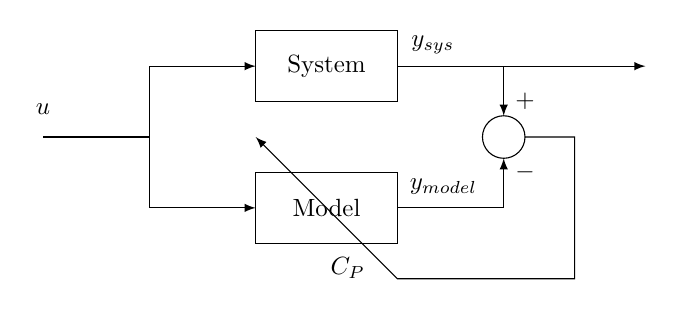
\begin{tikzpicture} [scale=0.9,transform shape]

\draw  (3,-1.5) rectangle (5,-2.5);
\node at (4,-2) {Model};

\draw  (3,0.5) rectangle (5,-0.5);
\node at (4,0) {System};

\node at (6.8,-1.5) {$-$};
\node at (5.5,0.3) {$y_{sys}$};
\node at (5.65,-1.7) {$y_{model}$};
\node at (4.3,-2.85) {$C_P$};
\node at (0,-0.6) {$u$};
\node at (6.8,-0.5) {$+$};

\draw  (6.5,-1) ellipse (0.3 and 0.3);

\draw [-latex](5,0) -- (8.5,0);
\draw [-latex](6.5,0) -- (6.5,-0.7);
\draw [-latex](1.5,-1) -- (1.5,0) -- (3,0);
\draw [-latex](1.5,-1) -- (1.5,-2) -- (3,-2);
\draw (0,-1) -- (1.5,-1);
\draw [-latex](5,-2) -- (6.5,-2) -- (6.5,-1.3);
\draw [-latex](6.8,-1) -- (7.5,-1) -- (7.5,-3) -- (5,-3) -- (3,-1);

\end{tikzpicture}% 
\caption{Parameter identification block diagram. }
\label{fig:parame_block}
\end{figure}

Applying KVL to the hydraulic model, the following expression is obtained: Moreover, the parameter estimation is carried out for steady-state 
situation where the inertia, $J$, will not act. Thus, the term containing the diagonal matrix $J$ can be disregarded from the equation. 

\begin{equation}
  0 = \pmb{B_1 \Delta p_1 }= \pmb{B_1} [ \pmb{J {B_1}}^T \pmb{\dot{z}} + f(\pmb{z},\pmb{ w}, \pmb{k_v})]  = \pmb{ B_1} (f(\pmb{z}, \pmb{w},\pmb{ k_v}))
  \label{esteq}
 \end{equation}
 
The pressure difference in the pumps have been specified as inputs, by reason of those pressures can be obtained from the setup available so they are considered 
as known parameters. Thereby, in \eqref{esteq} the term can be split up as following:
 
\begin{equation}
 0 = f(\pmb{z},\pmb{k_v})+ f(\pmb{z},\pmb{w})
 \label{ModelNoInertia}
\end{equation}

The term $f(\pmb{z},\pmb{w})$ is set as input, it is renamed as U and it represents the pressure difference in the $4$ pumps acting on the system. Therefore, 
\eqref{ModelNoInertia} is considered as the input equation where the flow through the chords and the friction parameter of the pipes are unknown. 

An output equation is defined, which represents the pressure difference known from the system setup. In this way, the output equation can be compared 
to the data measured in the setup and proceed to estimate the unknown parameters. 

From the system setup $8$ different relative pressures can be measured, following \figref{systemdiagram} notation the sensors are placed in: 
$n_2$ $n_4$ $n_5$ $n_7$ $n_{10}$ $n_{11}$ $n_{15}$ $n_{16}$.

In order to compare the measurements from the system setup and the data obtained from the simulation in Matlab, a reference point has to be set in the 
simulation to calculate the desired data. 

The atmospheric is set as reference point and the pressures obtained from the simulation are dependant on it. The relationship between pressures, where DpCXX describes
the pressure difference for the XX component, can be defined as:

\text{\underline{Node 2}} 
\vspace{4mm}
\begin{equation}
    DpC2 = y_1
\end{equation}

\text{\underline{Node 7}}
\vspace{4mm}
\begin{equation}
  DpC16 = y_2
\end{equation}

\text{\underline{Node 4}}
\vspace{4mm}
\begin {equation}
    DpC18 + DpC19 + DpC23 + DpC24 = y_3
\end{equation}

\text{\underline{Node 5}}
\vspace{4mm}
\begin {equation}
    DpC25 + DpC26 + DpC30 + DpC31 = y_4
\end{equation}

\text{\underline{Node 10}}
\vspace{4mm}
\begin {equation}
    DpC24 = y_5
\end{equation}

\text{\underline{Node 11}}
\vspace{4mm}
\begin {equation}
    DpC20 + DpC21= y_6
\end{equation}

\text{\underline{Node 15}}
\vspace{4mm}
\begin {equation}
    DpC31 = y_7
\end{equation}

\text{\underline{Node 16}}
\vspace{4mm}
\begin {equation}
    DpC28 + DpC27 = y_8
\end{equation}


With the $8$ equations depicted above the output vector $\pmb{y}$ is obtained. 

